\PassOptionsToPackage{unicode=true}{hyperref} % options for packages loaded elsewhere
\PassOptionsToPackage{hyphens}{url}
%
\documentclass[ignorenonframetext,]{beamer}
\usepackage{pgfpages}
\setbeamertemplate{caption}[numbered]
\setbeamertemplate{caption label separator}{: }
\setbeamercolor{caption name}{fg=normal text.fg}
\beamertemplatenavigationsymbolsempty
\usepackage{lmodern}
\usepackage{amssymb,amsmath}
\usepackage{ifxetex,ifluatex}
\usepackage{fixltx2e} % provides \textsubscript
\ifnum 0\ifxetex 1\fi\ifluatex 1\fi=0 % if pdftex
  \usepackage[T1]{fontenc}
  \usepackage[utf8]{inputenc}
  \usepackage{textcomp} % provides euro and other symbols
\else % if luatex or xelatex
  \usepackage{unicode-math}
  \defaultfontfeatures{Ligatures=TeX,Scale=MatchLowercase}
\fi
\usetheme[]{CambridgeUS}
\usecolortheme{beaver}
\usefonttheme{structurebold}
% use upquote if available, for straight quotes in verbatim environments
\IfFileExists{upquote.sty}{\usepackage{upquote}}{}
% use microtype if available
\IfFileExists{microtype.sty}{%
\usepackage[]{microtype}
\UseMicrotypeSet[protrusion]{basicmath} % disable protrusion for tt fonts
}{}
\IfFileExists{parskip.sty}{%
\usepackage{parskip}
}{% else
\setlength{\parindent}{0pt}
\setlength{\parskip}{6pt plus 2pt minus 1pt}
}
\usepackage{hyperref}
\hypersetup{
            pdftitle={Shapefiles},
            pdfauthor={Jan-Philipp Kolb},
            pdfborder={0 0 0},
            breaklinks=true}
\urlstyle{same}  % don't use monospace font for urls
\newif\ifbibliography
\usepackage{color}
\usepackage{fancyvrb}
\newcommand{\VerbBar}{|}
\newcommand{\VERB}{\Verb[commandchars=\\\{\}]}
\DefineVerbatimEnvironment{Highlighting}{Verbatim}{commandchars=\\\{\}}
% Add ',fontsize=\small' for more characters per line
\usepackage{framed}
\definecolor{shadecolor}{RGB}{248,248,248}
\newenvironment{Shaded}{\begin{snugshade}}{\end{snugshade}}
\newcommand{\AlertTok}[1]{\textcolor[rgb]{0.94,0.16,0.16}{#1}}
\newcommand{\AnnotationTok}[1]{\textcolor[rgb]{0.56,0.35,0.01}{\textbf{\textit{#1}}}}
\newcommand{\AttributeTok}[1]{\textcolor[rgb]{0.77,0.63,0.00}{#1}}
\newcommand{\BaseNTok}[1]{\textcolor[rgb]{0.00,0.00,0.81}{#1}}
\newcommand{\BuiltInTok}[1]{#1}
\newcommand{\CharTok}[1]{\textcolor[rgb]{0.31,0.60,0.02}{#1}}
\newcommand{\CommentTok}[1]{\textcolor[rgb]{0.56,0.35,0.01}{\textit{#1}}}
\newcommand{\CommentVarTok}[1]{\textcolor[rgb]{0.56,0.35,0.01}{\textbf{\textit{#1}}}}
\newcommand{\ConstantTok}[1]{\textcolor[rgb]{0.00,0.00,0.00}{#1}}
\newcommand{\ControlFlowTok}[1]{\textcolor[rgb]{0.13,0.29,0.53}{\textbf{#1}}}
\newcommand{\DataTypeTok}[1]{\textcolor[rgb]{0.13,0.29,0.53}{#1}}
\newcommand{\DecValTok}[1]{\textcolor[rgb]{0.00,0.00,0.81}{#1}}
\newcommand{\DocumentationTok}[1]{\textcolor[rgb]{0.56,0.35,0.01}{\textbf{\textit{#1}}}}
\newcommand{\ErrorTok}[1]{\textcolor[rgb]{0.64,0.00,0.00}{\textbf{#1}}}
\newcommand{\ExtensionTok}[1]{#1}
\newcommand{\FloatTok}[1]{\textcolor[rgb]{0.00,0.00,0.81}{#1}}
\newcommand{\FunctionTok}[1]{\textcolor[rgb]{0.00,0.00,0.00}{#1}}
\newcommand{\ImportTok}[1]{#1}
\newcommand{\InformationTok}[1]{\textcolor[rgb]{0.56,0.35,0.01}{\textbf{\textit{#1}}}}
\newcommand{\KeywordTok}[1]{\textcolor[rgb]{0.13,0.29,0.53}{\textbf{#1}}}
\newcommand{\NormalTok}[1]{#1}
\newcommand{\OperatorTok}[1]{\textcolor[rgb]{0.81,0.36,0.00}{\textbf{#1}}}
\newcommand{\OtherTok}[1]{\textcolor[rgb]{0.56,0.35,0.01}{#1}}
\newcommand{\PreprocessorTok}[1]{\textcolor[rgb]{0.56,0.35,0.01}{\textit{#1}}}
\newcommand{\RegionMarkerTok}[1]{#1}
\newcommand{\SpecialCharTok}[1]{\textcolor[rgb]{0.00,0.00,0.00}{#1}}
\newcommand{\SpecialStringTok}[1]{\textcolor[rgb]{0.31,0.60,0.02}{#1}}
\newcommand{\StringTok}[1]{\textcolor[rgb]{0.31,0.60,0.02}{#1}}
\newcommand{\VariableTok}[1]{\textcolor[rgb]{0.00,0.00,0.00}{#1}}
\newcommand{\VerbatimStringTok}[1]{\textcolor[rgb]{0.31,0.60,0.02}{#1}}
\newcommand{\WarningTok}[1]{\textcolor[rgb]{0.56,0.35,0.01}{\textbf{\textit{#1}}}}
\usepackage{longtable,booktabs}
\usepackage{caption}
% These lines are needed to make table captions work with longtable:
\makeatletter
\def\fnum@table{\tablename~\thetable}
\makeatother
\usepackage{graphicx,grffile}
\makeatletter
\def\maxwidth{\ifdim\Gin@nat@width>\linewidth\linewidth\else\Gin@nat@width\fi}
\def\maxheight{\ifdim\Gin@nat@height>\textheight\textheight\else\Gin@nat@height\fi}
\makeatother
% Scale images if necessary, so that they will not overflow the page
% margins by default, and it is still possible to overwrite the defaults
% using explicit options in \includegraphics[width, height, ...]{}
\setkeys{Gin}{width=\maxwidth,height=\maxheight,keepaspectratio}
% Prevent slide breaks in the middle of a paragraph:
\widowpenalties 1 10000
\raggedbottom
\setbeamertemplate{part page}{
\centering
\begin{beamercolorbox}[sep=16pt,center]{part title}
  \usebeamerfont{part title}\insertpart\par
\end{beamercolorbox}
}
\setbeamertemplate{section page}{
\centering
\begin{beamercolorbox}[sep=12pt,center]{part title}
  \usebeamerfont{section title}\insertsection\par
\end{beamercolorbox}
}
\setbeamertemplate{subsection page}{
\centering
\begin{beamercolorbox}[sep=8pt,center]{part title}
  \usebeamerfont{subsection title}\insertsubsection\par
\end{beamercolorbox}
}
\AtBeginPart{
  \frame{\partpage}
}
\AtBeginSection{
  \ifbibliography
  \else
    \frame{\sectionpage}
  \fi
}
\AtBeginSubsection{
  \frame{\subsectionpage}
}
\setlength{\emergencystretch}{3em}  % prevent overfull lines
\providecommand{\tightlist}{%
  \setlength{\itemsep}{0pt}\setlength{\parskip}{0pt}}
\setcounter{secnumdepth}{0}

% set default figure placement to htbp
\makeatletter
\def\fps@figure{htbp}
\makeatother


\title{Shapefiles}
\author{Jan-Philipp Kolb}
\date{23 Oktober 2018}

\begin{document}
\frame{\titlepage}

\begin{frame}{Worum geht es in diesem Abschnitt}
\protect\hypertarget{worum-geht-es-in-diesem-abschnitt}{}

\begin{itemize}
\tightlist
\item
  Shapefiles mit Vorwahl- und PLZ-Bereichen importieren
\item
  PLZ-Bereiche zusammenfassen
\item
  Eine räumliche Stichprobe ziehen
\item
  Adressen für die gezogenen Punkte bestimmen
\item
  Adressdatensatz bereinigen
\item
  Entfernung zum Hauptbahnhof bestimmen
\end{itemize}

\end{frame}

\begin{frame}[fragile]{Ortsnetzbereiche}
\protect\hypertarget{ortsnetzbereiche}{}

Quelle:
\href{http://www.bundesnetzagentur.de/DE/Sachgebiete/Telekommunikation/Unternehmen_Institutionen/Nummerierung/Rufnummern/ONVerzeichnisse/GISDaten_ONBGrenzen/ONBGrenzen_Basepage.html}{Bundesnetzagentur}

\begin{Shaded}
\begin{Highlighting}[]
\KeywordTok{setwd}\NormalTok{(}\StringTok{"D:/Daten/Daten/GeoDaten/"}\NormalTok{)}
\KeywordTok{library}\NormalTok{(maptools)}
\NormalTok{onb <-}\StringTok{ }\KeywordTok{readShapePoly}\NormalTok{(}\StringTok{"onb_grenzen.shp"}\NormalTok{)}
\end{Highlighting}
\end{Shaded}

\end{frame}

\begin{frame}{Die Karte zeichnen}
\protect\hypertarget{die-karte-zeichnen}{}

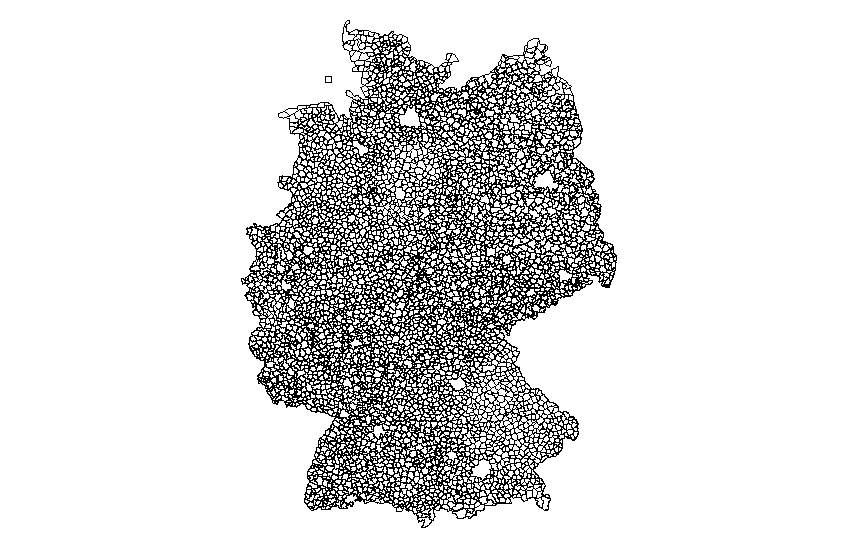
\includegraphics{figure/onbGermany.png}

\end{frame}

\begin{frame}{Einen Vorwahlbereich ausschneiden}
\protect\hypertarget{einen-vorwahlbereich-ausschneiden}{}

\end{frame}

\begin{frame}{Vorwahlbereich ausschneiden}
\protect\hypertarget{vorwahlbereich-ausschneiden}{}

\end{frame}

\begin{frame}{Shapefiles zusammenfassen}
\protect\hypertarget{shapefiles-zusammenfassen}{}

\end{frame}

\begin{frame}[fragile]{PLZ Datensatz einlesen}
\protect\hypertarget{plz-datensatz-einlesen}{}

\begin{itemize}
\tightlist
\item
  \href{http://arnulf.us/PLZ}{\textbf{Quelle}} für PLZ Shapefiles
\end{itemize}

\begin{verbatim}
## Loading required package: sp
\end{verbatim}

\begin{verbatim}
## rgdal: version: 1.3-2, (SVN revision 755)
##  Geospatial Data Abstraction Library extensions to R successfully loaded
##  Loaded GDAL runtime: GDAL 2.2.3, released 2017/11/20
##  Path to GDAL shared files: D:/Eigene Dateien/Dokumente/R/win-library/3.5/rgdal/gdal
##  GDAL binary built with GEOS: TRUE 
##  Loaded PROJ.4 runtime: Rel. 4.9.3, 15 August 2016, [PJ_VERSION: 493]
##  Path to PROJ.4 shared files: D:/Eigene Dateien/Dokumente/R/win-library/3.5/rgdal/proj
##  Linking to sp version: 1.3-1
\end{verbatim}

\begin{verbatim}
## OGR data source with driver: ESRI Shapefile 
## Source: "D:\GESIS\data\post_pl.shp", layer: "post_pl"
## with 8270 features
## It has 3 fields
\end{verbatim}

\end{frame}

\begin{frame}{Die Daten plotten}
\protect\hypertarget{die-daten-plotten}{}

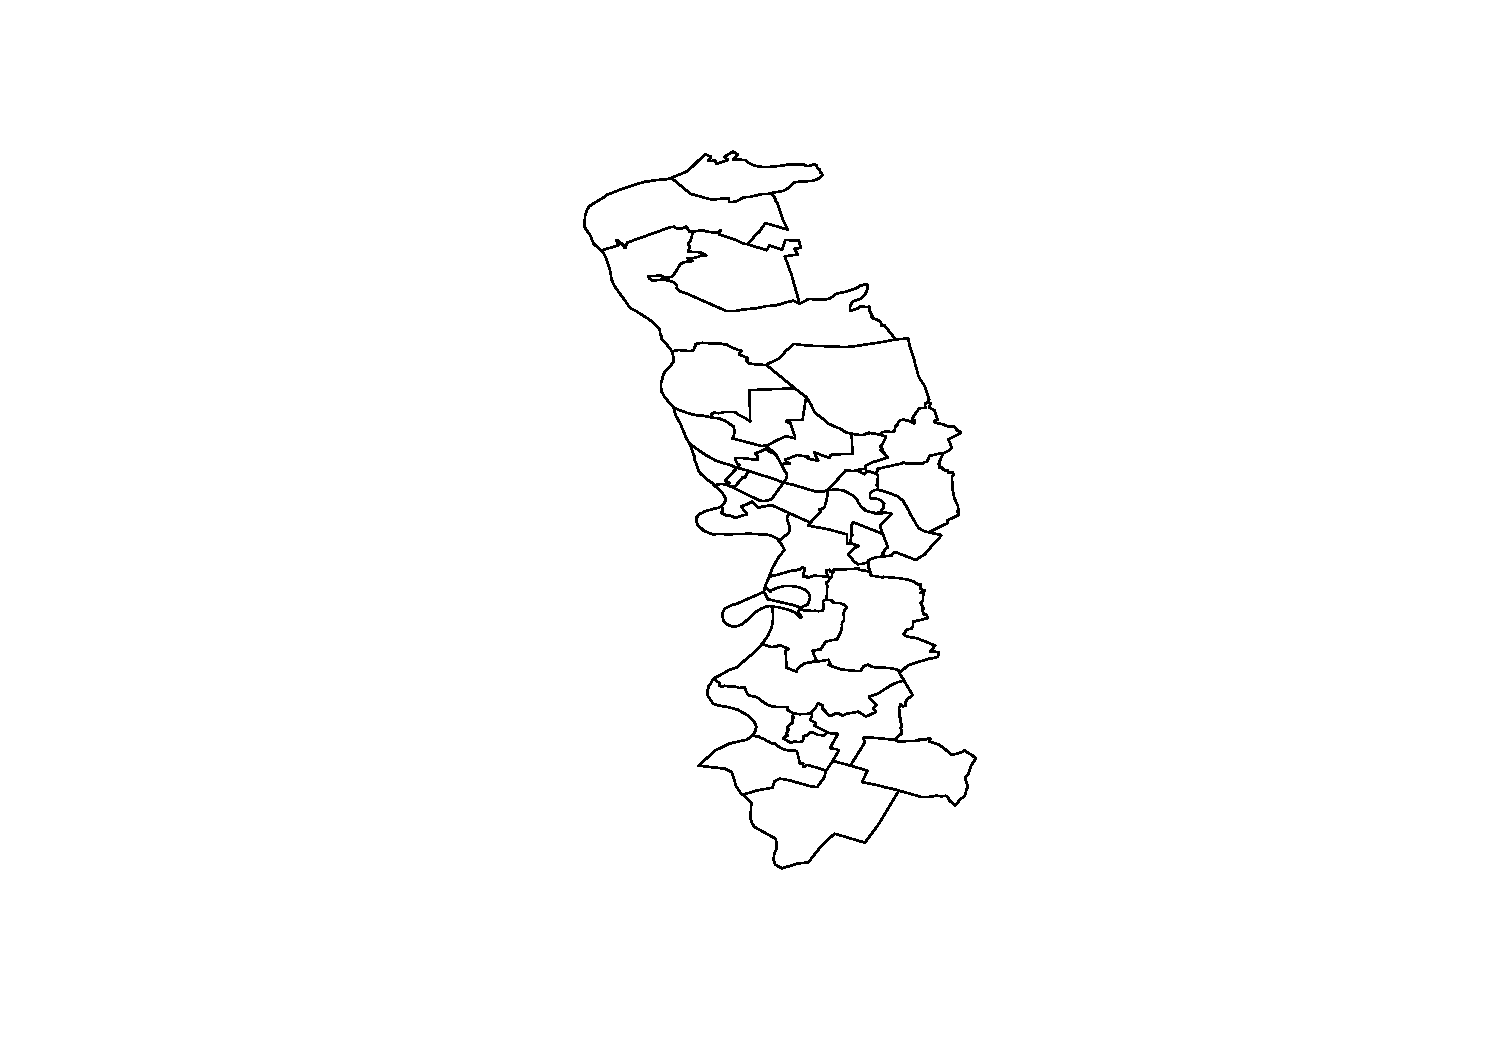
\includegraphics{Shapefiles_files/figure-beamer/unnamed-chunk-11-1.pdf}

\end{frame}

\begin{frame}{Die Grenze von Mannheim}
\protect\hypertarget{die-grenze-von-mannheim}{}

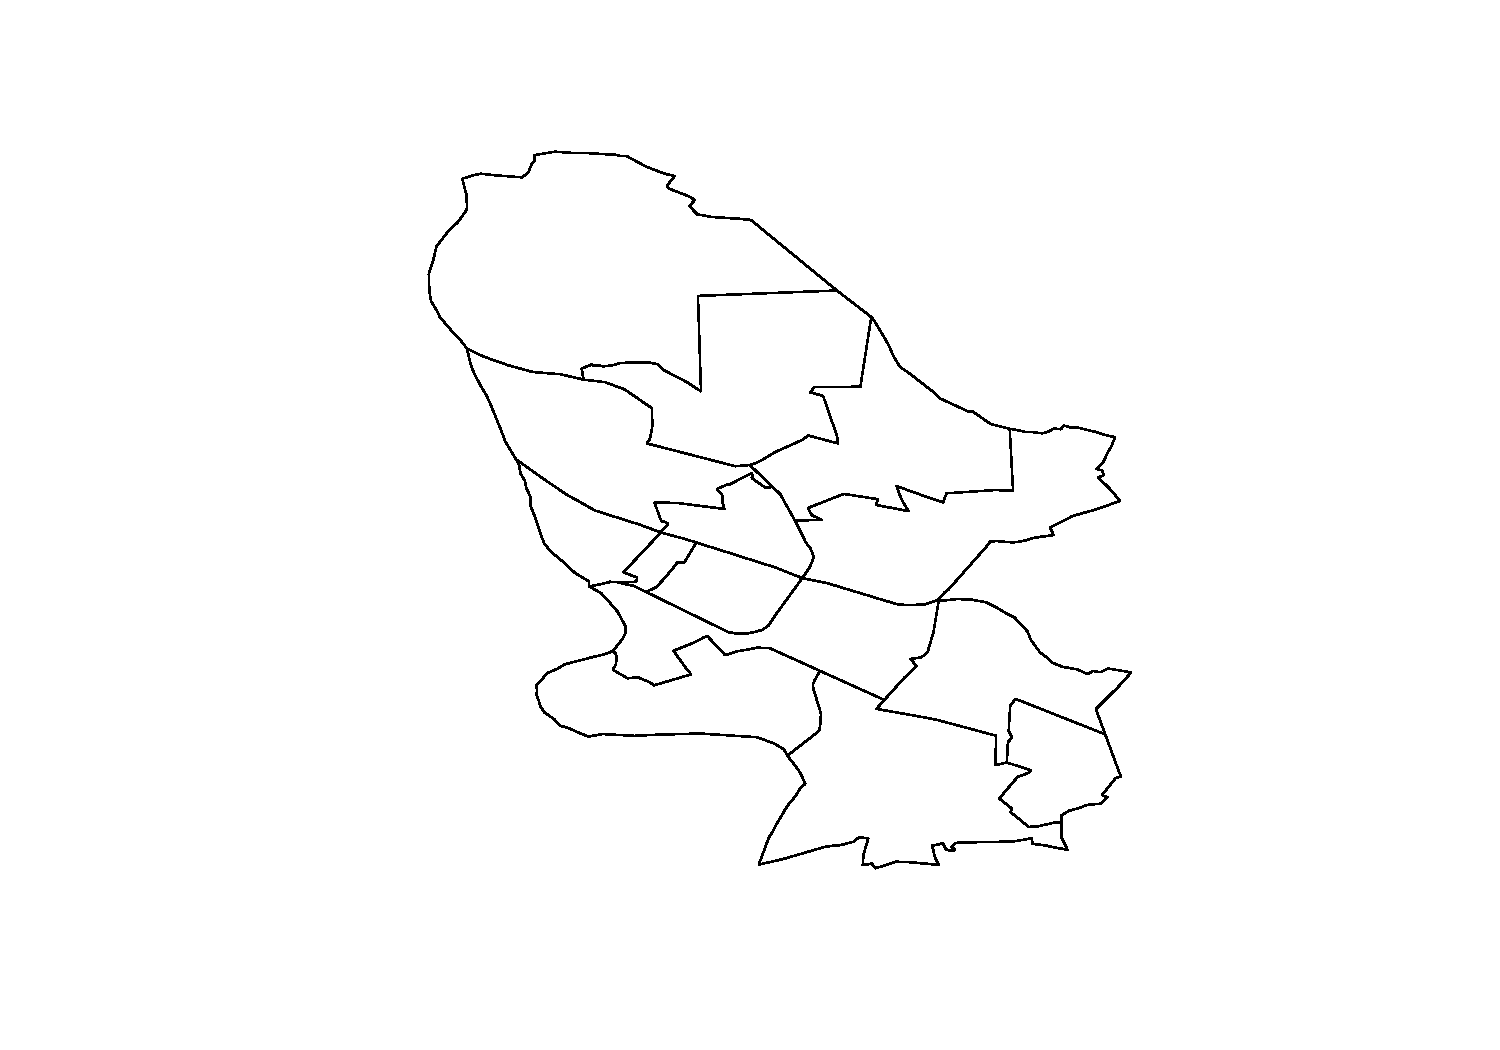
\includegraphics{Shapefiles_files/figure-beamer/unnamed-chunk-12-1.pdf}

\end{frame}

\begin{frame}[fragile]{Die PLZ-Bereiche von Mannheim zusammenfassen}
\protect\hypertarget{die-plz-bereiche-von-mannheim-zusammenfassen}{}

\begin{itemize}
\tightlist
\item
  Wir nutzen den Befehl \texttt{unionSpatialPolygons} im Paket
  \texttt{maptools}
\end{itemize}

\begin{verbatim}
## Checking rgeos availability: TRUE
\end{verbatim}


\includegraphics{Shapefiles_files/figure-beamer/unnamed-chunk-13-1.pdf}

\end{frame}

\begin{frame}{Der Grenze von Deutschland}
\protect\hypertarget{der-grenze-von-deutschland}{}

\end{frame}

\begin{frame}{\href{https://www.rdocumentation.org/packages/sp/versions/1.3-1/topics/spsample}{Räumliche
Stichprobe}}
\protect\hypertarget{raumliche-stichprobe}{}

\end{frame}

\begin{frame}[fragile]{Reverse Geokodierung}
\protect\hypertarget{reverse-geokodierung}{}

\begin{verbatim}
## Loading required package: ggplot2
\end{verbatim}

\begin{verbatim}
## Warning: package 'ggplot2' was built under R version 3.5.1
\end{verbatim}

\end{frame}

\begin{frame}{Die räumliche Stichprobe plotten}
\protect\hypertarget{die-raumliche-stichprobe-plotten}{}

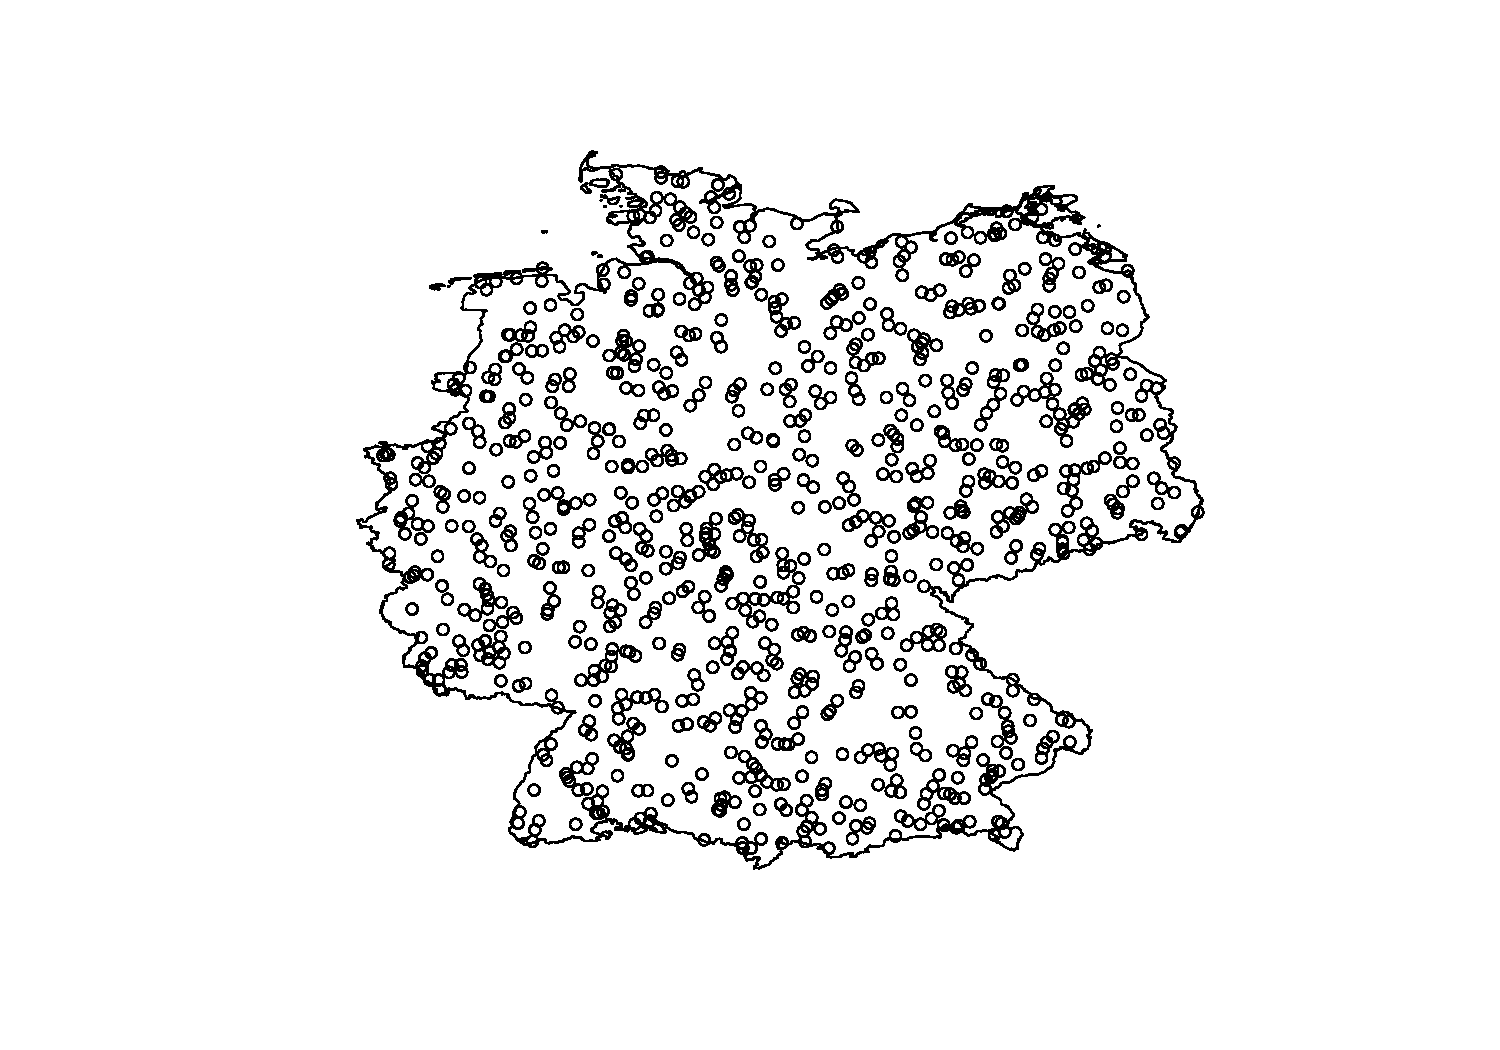
\includegraphics{Shapefiles_files/figure-beamer/unnamed-chunk-21-1.pdf}

\end{frame}

\begin{frame}{Nur tatsächliche Adressen}
\protect\hypertarget{nur-tatsachliche-adressen}{}

\begin{itemize}
\tightlist
\item
  \href{http://stat545.com/block022_regular-expression.html}{\textbf{Reguläre
  Ausdrücke}} in R
\end{itemize}

\end{frame}

\begin{frame}{Das Ergebnis plotten}
\protect\hypertarget{das-ergebnis-plotten}{}

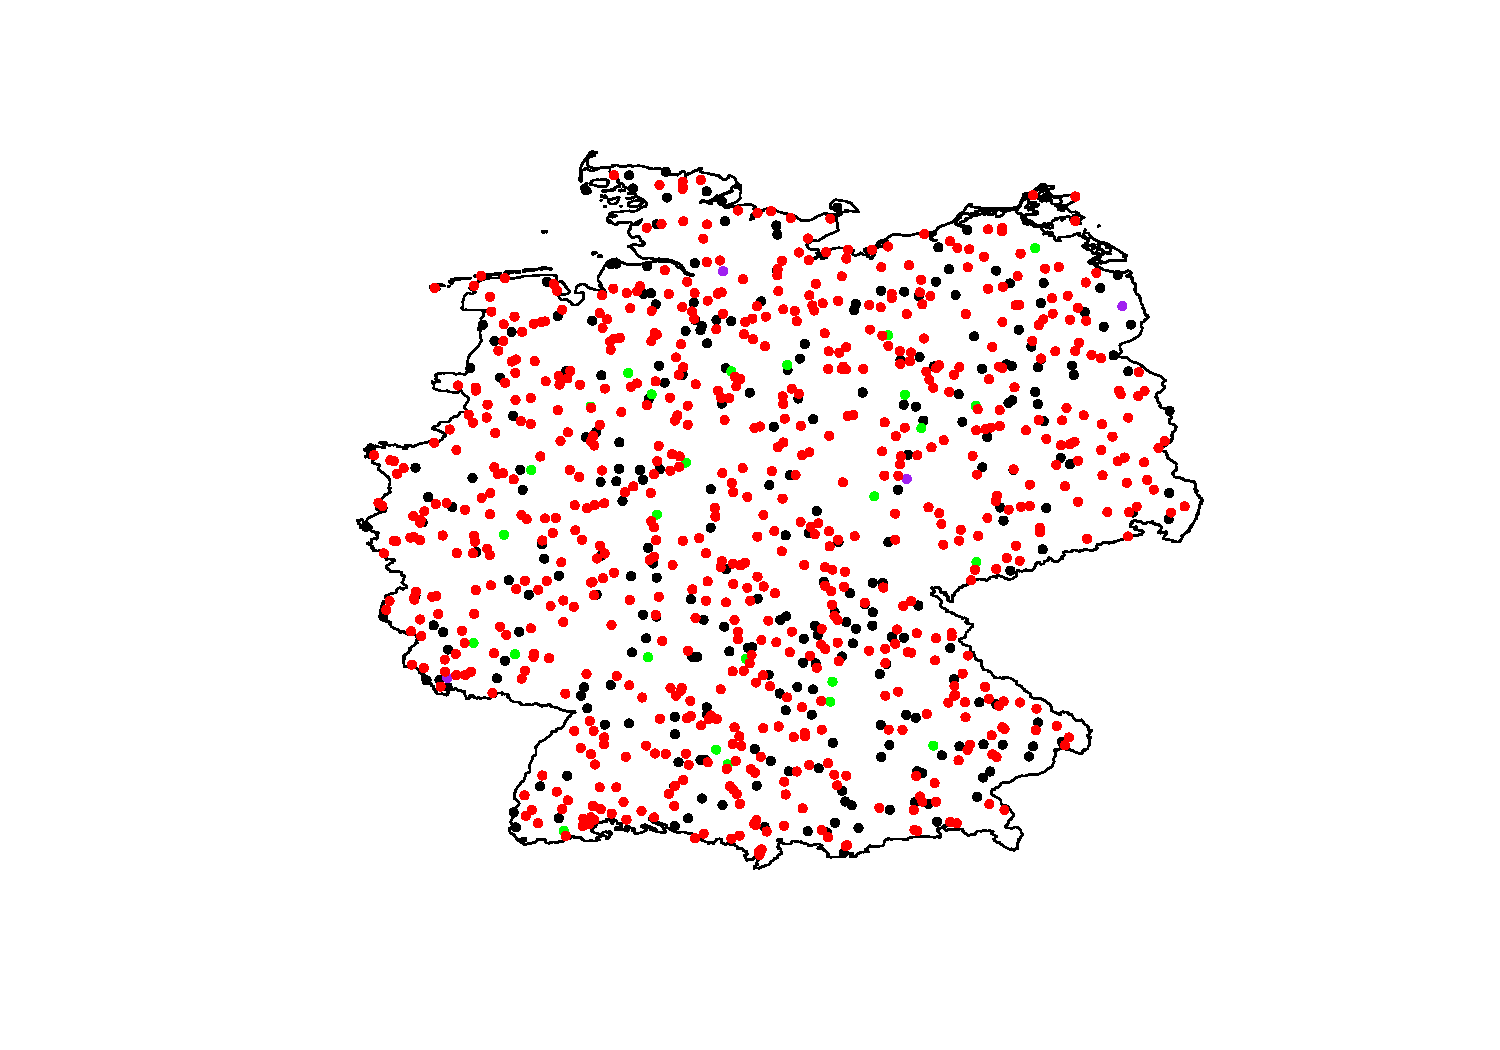
\includegraphics{Shapefiles_files/figure-beamer/unnamed-chunk-24-1.pdf}

\end{frame}

\begin{frame}[fragile]{Distanzen berechnen}
\protect\hypertarget{distanzen-berechnen}{}

\begin{verbatim}
## starting httpd help server ... done
\end{verbatim}

\end{frame}

\begin{frame}{Das shapefile Format \ldots{}}
\protect\hypertarget{das-shapefile-format}{}

\begin{itemize}
\item
  \ldots{} ist ein beliebtes Format räumlicher Vektordaten für
  geographisches Informationssysteme (GIS).
\item
  Es wurde entwickelt und reguliert von
  \href{http://www.esri.com/}{ESRI}
\item
  (meist) offene Spezifikation um Daten Interoperabilität zwischen Esri
  und anderen Formaten zu sichern.
\item
  Es können Punkte, Linien und Polygone beschrieben werden
\item
  Jedes Element hat Attribute, wie bspw. Name oder Temperatur die es
  beschreiben.
\end{itemize}

Quelle: \url{https://en.wikipedia.org/wiki/Shapefile}

\end{frame}

\begin{frame}{Global Adminastrative Boundaries -
\href{http://www.gadm.org/}{GADM} - NUTS level 1}
\protect\hypertarget{global-adminastrative-boundaries---gadm---nuts-level-1}{}


\includegraphics{Shapefiles_files/figure-beamer/unnamed-chunk-29-1.pdf}

\end{frame}

\begin{frame}[fragile]{Ein Blick auf die Daten}
\protect\hypertarget{ein-blick-auf-die-daten}{}

Koordinaten im polygon slot

\begin{verbatim}
##          [,1]     [,2]
## [1,] 6.026519 50.17767
## [2,] 6.031361 50.16563
## [3,] 6.035646 50.16410
## [4,] 6.042747 50.16157
## [5,] 6.043894 50.16116
## [6,] 6.048243 50.16008
\end{verbatim}

\end{frame}

\begin{frame}[fragile]{Der Datenslot}
\protect\hypertarget{der-datenslot}{}

\begin{verbatim}
##   OBJECTID ID_0 ISO     NAME_0 ID_1       NAME_1 HASC_1 CCN_1 CCA_1
## 1        1  131 LUX Luxembourg    1     Diekirch  LU.DI    NA      
## 2        2  131 LUX Luxembourg    2 Grevenmacher  LU.GR    NA      
## 3        3  131 LUX Luxembourg    3   Luxembourg  LU.LU    NA      
##     TYPE_1 ENGTYPE_1 NL_NAME_1            VARNAME_1
## 1 District  District               Dikrech|Dikkrich
## 2 District  District                  Gréivemaacher
## 3 District  District           Lëtzebuerg|Luxemburg
\end{verbatim}

\end{frame}

\begin{frame}{\href{http://www.gadm.org/}{GADM}- NUTS level 3}
\protect\hypertarget{gadm--nuts-level-3}{}

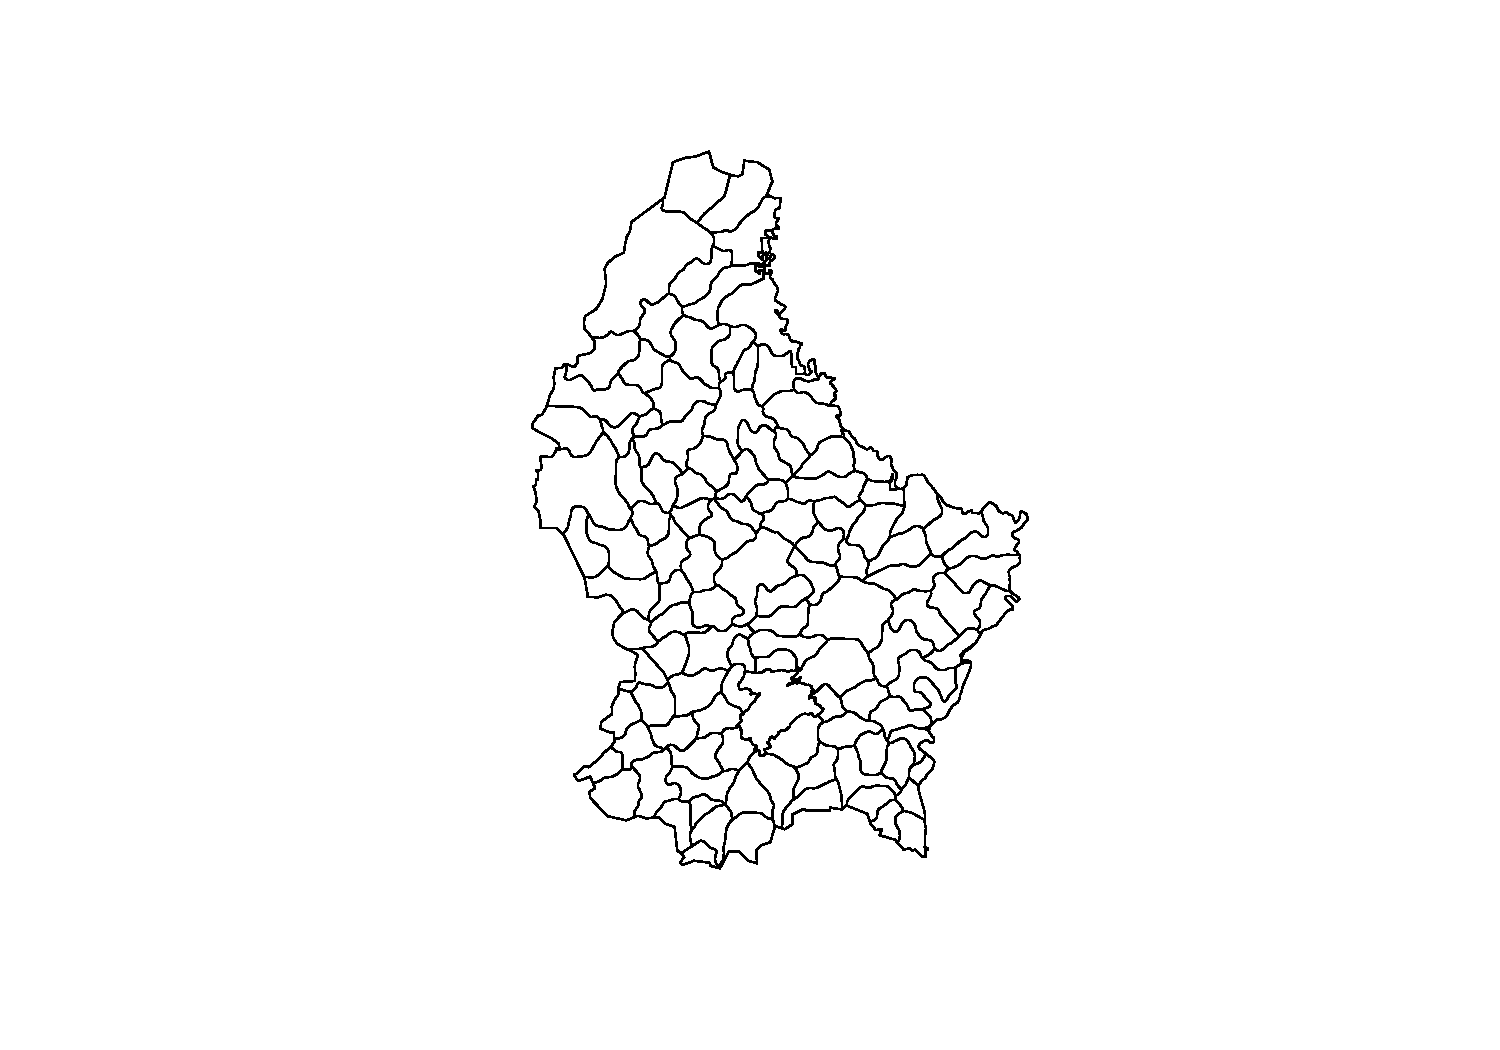
\includegraphics{Shapefiles_files/figure-beamer/LUX3-1.pdf}

\end{frame}

\begin{frame}{\href{http://www.gadm.org/}{GADM}- NUTS level 4}
\protect\hypertarget{gadm--nuts-level-4}{}


\includegraphics{Shapefiles_files/figure-beamer/LUX4-1.pdf}

\end{frame}

\begin{frame}{\href{http://www.gadm.org/}{GADM}- NUTS level 3}
\protect\hypertarget{gadm--nuts-level-3-1}{}

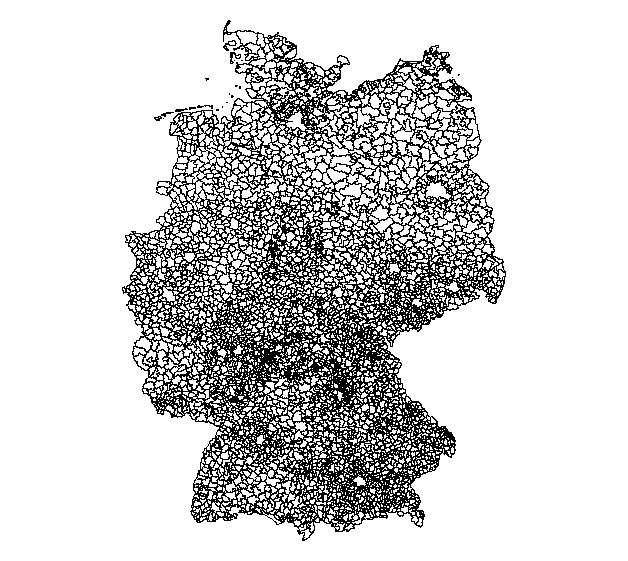
\includegraphics{figure/DEU3.png}

\end{frame}

\begin{frame}[fragile]{PLZ für Deutschland}
\protect\hypertarget{plz-fur-deutschland}{}

\begin{itemize}
\item
  \url{http://datahub.io/de/dataset/postal-codes-de}
\item
  datahub.io funktioniert leider nicht mehr
\item
  \url{http://arnulf.us/PLZ}
\end{itemize}

\begin{Shaded}
\begin{Highlighting}[]
\NormalTok{PLZ <-}\StringTok{ }\KeywordTok{readOGR}\NormalTok{ (}\StringTok{"post_pl.shp"}\NormalTok{,}\StringTok{"post_pl"}\NormalTok{)}
\end{Highlighting}
\end{Shaded}

\end{frame}

\begin{frame}{Der R Befehl readShapePoly}
\protect\hypertarget{der-r-befehl-readshapepoly}{}

Um Shape-Dateien zu lesen, ist es notwendig, die drei Dateien mit den
folgenden Dateierweiterungen im gleichen Verzeichnis zu haben:

\begin{itemize}
\tightlist
\item
  .shp
\item
  .dbf
\item
  .shx
\end{itemize}

\end{frame}

\begin{frame}{Mannheim zeichnen}
\protect\hypertarget{mannheim-zeichnen}{}

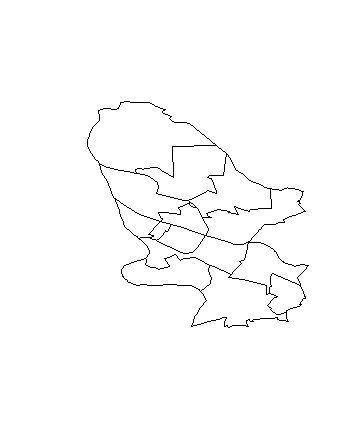
\includegraphics{https://raw.githubusercontent.com/Japhilko/GeoData/master/2016/slides/figure/MannheimPLZ.png}

\end{frame}

\begin{frame}{Gemeinden in Deutschland}
\protect\hypertarget{gemeinden-in-deutschland}{}

\href{http://www.geodatenzentrum.de/geodaten/gdz_rahmen.gdz_div?gdz_spr=deu\&gdz_akt_zeile=5\&gdz_anz_zeile=1\&gdz_unt_zeile=15\&gdz_user_id=0}{Bundesamt
für Kartographie und Geodäsie (BKG)}

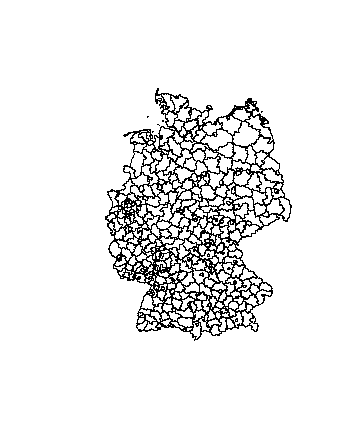
\includegraphics{figure/vg250_krs.png}

\end{frame}

\begin{frame}{Kreise eines Bundeslandes}
\protect\hypertarget{kreise-eines-bundeslandes}{}

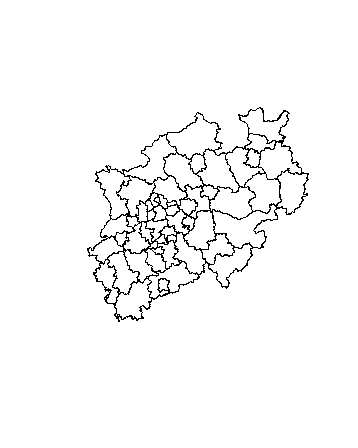
\includegraphics{figure/KreiseNRW.png}

\end{frame}

\begin{frame}{\href{http://www.bundesnetzagentur.de/SharedDocs/Downloads/DE/Sachgebiete/Telekommunikation/Unternehmen_Institutionen/Nummerierung/Rufnummern/ONVerzeichnisse/ONBGrenzen/ONB_Grenzen.html}{Vorwahlbereiche
in Deutschland}}
\protect\hypertarget{vorwahlbereiche-in-deutschland}{}

\url{http://www.bundesnetzagentur.de/}

\begin{longtable}[]{@{}llll@{}}
\toprule
& VORWAHL & NAME & KENNUNG\tabularnewline
\midrule
\endhead
0 & 04651 & Sylt & NA\tabularnewline
1 & 04668 & Klanxbüll & NA\tabularnewline
2 & 04664 & Neukirchen b Niebüll & NA\tabularnewline
3 & 04663 & Süderlügum & NA\tabularnewline
4 & 04666 & Ladelund & NA\tabularnewline
5 & 04631 & Glücksburg Ostsee & NA\tabularnewline
\bottomrule
\end{longtable}

\end{frame}

\begin{frame}{Vorwahlbereich 06}
\protect\hypertarget{vorwahlbereich-06}{}

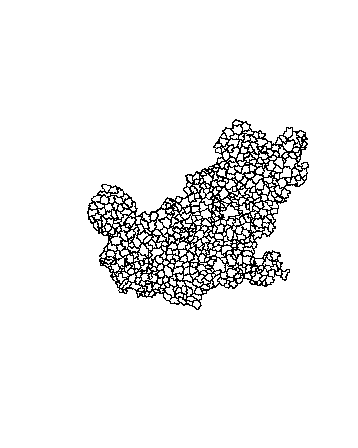
\includegraphics{figure/Vorwahl06.png}

\end{frame}

\begin{frame}{Wo ist Mannheim?}
\protect\hypertarget{wo-ist-mannheim}{}

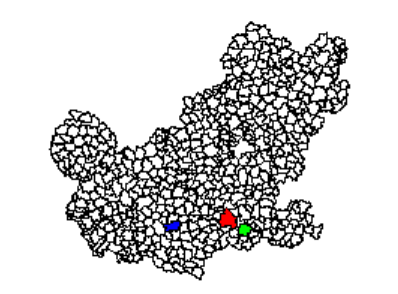
\includegraphics{figure/DreiStaedte.png}

\end{frame}

\begin{frame}[fragile]{Andere Quellen}
\protect\hypertarget{andere-quellen}{}

\begin{itemize}
\tightlist
\item
  \href{http://msi.nga.mil/NGAPortal/MSI.portal?_nfpb=true\&_pageLabel=msi_portal_page_62\&pubCode=0015}{World
  Port Index}
\end{itemize}

\begin{Shaded}
\begin{Highlighting}[]
\KeywordTok{library}\NormalTok{(rgdal)}
\NormalTok{WPI <-}\StringTok{ }\KeywordTok{readOGR}\NormalTok{ (}\StringTok{"WPI.shp"}\NormalTok{,}\StringTok{"WPI"}\NormalTok{)}
\KeywordTok{plot}\NormalTok{(WPI)}
\end{Highlighting}
\end{Shaded}


\includegraphics{figure/WPI.png}

Datenbanken für Karten

\end{frame}

\begin{frame}{Weitere Quellen}
\protect\hypertarget{weitere-quellen}{}

\begin{itemize}
\item
  \href{http://epp.eurostat.ec.europa.eu/portal/page/portal/gisco_Geographical_information_maps/popups/\%20references/administrative_units_statistical_units_1}{Eurostat
  Karten}
\item
  \href{https://www.ordnancesurvey.co.uk/business-and-government/products/opendata-products-grid.html}{Open
  linked data}
\item
  \href{http://thematicmapping.org/downloads/world_borders.php}{World
  Borders Datensatz}
\item
  \href{https://www.nhgis.org/}{National Historical Information System}
\item
  \href{http://www.freemapdata.com/html/free_polygon_data.html}{Freie
  polygon Daten für die USA}
\item
  \href{https://science.nature.nps.gov/im/datamgmt/statistics/r/advanced/spatial.cfm}{Spatial
  Data in R}
\item
  \href{http://www.r-bloggers.com/shapefile-polygons-plotted-on-google-maps-using-ggmap-in-r-throw-some-throw-some-stats-on-that-mappart-2/}{ggmap
  und shapefiles}
\end{itemize}

\end{frame}

\end{document}
